% !TeX root = ../thuthesis-example.tex

\chapter{API优先开发}

API优先开发(API-First Development)是一种软件设计与开发方法论,其核心在于在实际开发前,先完成应用程序接口(Application Programming Interface, API)的设计与定义。与传统开发模式相比,API优先开发将接口设计置于开发流程前端,作为系统架构和功能实现的基础。在此模式下,开发团队首先创建API规范(通常基于OpenAPI/Swagger标准),明确定义接口资源、端点、请求方法、参数、响应格式及认证机制等要素。

bolt.se的APIActions模块是API优先理念的具体实现,允许用户定义和管理外部API,并使大语言模型(Large Language Model, LLM)能够理解并调用这些API扩展功能。本章将介绍API优先开发的概念、意义、优势、对LLM驱动软件开发的重要性,以及bolt.se中APIActions的实现方案。

\section{API优先开发的概念与意义}

\subsection{API优先开发在软件工程中的优势}
API优先开发为现代软件工程带来了以下优势:

\begin{enumerate}
  \item \textbf{并行开发效率}:明确的API规范使前端、后端和移动端团队能够在实际实现前达成共识,支持并行开发,减少集成阶段的冲突和返工。
  
  \item \textbf{一致性与标准化}:统一的API设计确保系统各服务接口的一致性,简化学习曲线,降低维护成本。
  
  \item \textbf{模块化与解耦}:以API为界面的系统设计促进高内聚低耦合架构,各服务或模块只需关注自身API的实现和消费,不必了解其他组件内部逻辑。
  
  \item \textbf{可测试性增强}:明确的API规范支持在实现前进行接口测试设计,有利于自动化测试和契约测试的实施。
  
  \item \textbf{文档驱动开发}:API规范自然成为系统技术文档,减少文档滞后或不准确问题,提高开发效率。
\end{enumerate}

在bolt.se等现代开发平台中,API优先方法有效减少沟通成本,避免设计误解,提早发现设计缺陷,从而提升开发团队效率和产品质量。

\subsection{API优先开发对LLM驱动软件开发的重要性}
在LLM驱动的软件开发范式中,API优先开发具有特殊意义:

\begin{enumerate}
  \item \textbf{结构化信息交互}:LLM与外部系统交互需要明确的结构和规范。API定义为LLM提供了调用外部服务的蓝图,避免了模糊指令导致的错误。
  
  \item \textbf{功能扩展}:通过API集成,LLM可突破知识截止限制,访问实时数据、专业工具和特定领域服务,扩展其能力边界。
  
  \item \textbf{权限控制}:API定义中的认证和授权机制为LLM提供受控访问方式,确保其操作在安全合规边界内执行。
  
  \item \textbf{工具智能}(Tool Intelligence):预定义API使LLM能理解可用工具的能力和限制,做出合理的工具选择和调用决策。
  
  \item \textbf{组合能力}:API优先开发支持LLM与多种服务和工具的组合使用,使复杂任务可分解为多个API调用的组合,增强问题解决能力。
\end{enumerate}

bolt.se深度融合API优先理念,通过将OpenAPI规范集成到开发流程中,实现LLM与外部API的无缝协作,使开发者能通过自然语言交互获得API增强的智能辅助。bolt.se的APIActions模块作为此理念的实现,结合了LLM的灵活性与API的精确性和功能扩展性,为软件开发带来显著效率提升。

\section{OpenAPI规范与API设计}
OpenAPI规范(原Swagger规范)是API优先开发的核心技术支撑,为API描述和交互提供了标准化、语言无关的格式\cite{openapi2023}。作为业界广泛采用的API定义标准,OpenAPI使开发者能以声明式方式完整定义API的各方面,实现从设计到实现、测试和文档的全生命周期管理。

OpenAPI规范采用JSON或YAML格式,结构化描述API的端点(endpoints)、操作(operations)、参数、响应、认证方法等关键要素。这种规范不仅适合人类理解,也便于机器处理,成为前端、后端和各类工具间沟通的桥梁。

在LLM驱动的开发环境中,OpenAPI规范定义RESTful API调用说明,从而更高效地利用现有功能,避免重复开发,并降低模型token使用。结构化API定义使大模型能够:
\begin{enumerate}
  \item 准确理解API功能和用法,无需详细自然语言解释
  \item 通过调用现有API获取数据,而非生成可能不准确的信息
  \item 避免在上下文中包含冗长API使用说明,节省token空间
  \item 将复杂任务分解为定义明确的API调用序列,提高解决效率
\end{enumerate}

\subsection{OpenAPI规范简介}
OpenAPI规范是结构化的API描述格式,主要包含以下组成部分\cite{openapi2023spec}:

\begin{enumerate}
  \item \textbf{基本信息}:API的标题、描述、版本、联系人信息和许可证等元数据。
  
  \item \textbf{服务器信息}:API的基础URL和不同环境(开发、测试、生产)的服务器地址。
  
  \item \textbf{路径}:API的各端点及可用HTTP方法(GET、POST、PUT、DELETE等),是规范核心部分。
  
  \item \textbf{组件}:包含可重用部分:
    \begin{itemize}
      \item \textit{schemas}:API使用的数据模型和对象结构。
      \item \textit{parameters}:可重用的参数定义。
      \item \textit{responses}:各种响应格式和状态码。
      \item \textit{securitySchemes}:API支持的安全认证机制。
    \end{itemize}
  
  \item \textbf{操作}:每个API端点的可用操作,包括:
    \begin{itemize}
      \item 操作ID与摘要,用于工具和代码生成。
      \item 描述与标签,用于文档组织。
      \item 参数定义(路径、查询、头部、cookie等)。
      \item 请求体结构与格式。
      \item 可能的响应状态与内容。
      \item 所需安全机制。
    \end{itemize}
\end{enumerate}

以下是bolt.se中支持的OpenAPI定义示例,展示一个简单的天气API:

\begin{verbatim}
openapi: 3.0.0
info:
  title: Weather API
  version: 1.0.0
servers:
  - url: https://api.weather.gov
    description: Weather API Server
paths:
  /weather/current:
    get:
      summary: Get current weather
      parameters:
        - name: city
          in: query
          required: true
          schema:
            type: string
      responses:
        '200':
          description: Current weather data
          content:
            application/json:
              schema:
                type: object
                properties:
                  temperature:
                    type: number
                  conditions:
                    type: string
\end{verbatim}

bolt.se的APIActions模块解析这类OpenAPI定义,提取API端点和操作,使LLM能理解并正确调用这些API。

\subsection{使用OpenAPI规范进行API设计的优势}
在bolt.se等现代开发环境中,采用OpenAPI规范进行API设计带来多方面优势:

\begin{enumerate}
  \item \textbf{设计驱动开发}:OpenAPI规范促使开发者在编码前先思考接口设计,从需求和用户体验出发设计API,避免实现细节对接口设计的不当影响。
  
  \item \textbf{自动化代码生成}:基于OpenAPI规范,bolt.se可帮助开发者生成调用API的代码片段,减少重复编码工作。
  
  \item \textbf{交互式使用}:bolt.se将OpenAPI规范转化为可交互形式,使用户能通过自然语言直接调用这些API,无需编写复杂代码。
    
  \item \textbf{机器可读性}:规范的结构化特性使LLM能理解和分析API,为智能开发辅助、代码补全和自动化请求提供基础。
\end{enumerate}

在bolt.se中,OpenAPI规范的机器可读特性具有重要价值。LLM可基于规范生成准确的API调用代码,理解API功能边界,甚至提供API使用建议。同时,规范中明确的数据模型和参数约束有助于LLM生成更准确的代码和请求,减少错误。

bolt.se的APIActions模块不仅用于定义系统内部服务接口,也作为用户自定义外部API的标准格式。通过解析OpenAPI文档为系统理解的API操作集,bolt.se实现了LLM直接利用这些API进行交互和代码生成,展示了API优先理念与AI驱动开发的融合。

\section{bolt.se中的APIActions实现}
bolt.se作为AI驱动的软件开发平台,将API优先开发理念融入其架构设计。系统通过APIActions模块,使用户能够定义、管理和应用外部API,同时使LLM能理解并调用这些API,实现功能扩展和技术集成。本节介绍bolt.se中APIActions的实现方案,从整体架构到具体功能实现。

\begin{figure}[htbp]
  \centering
  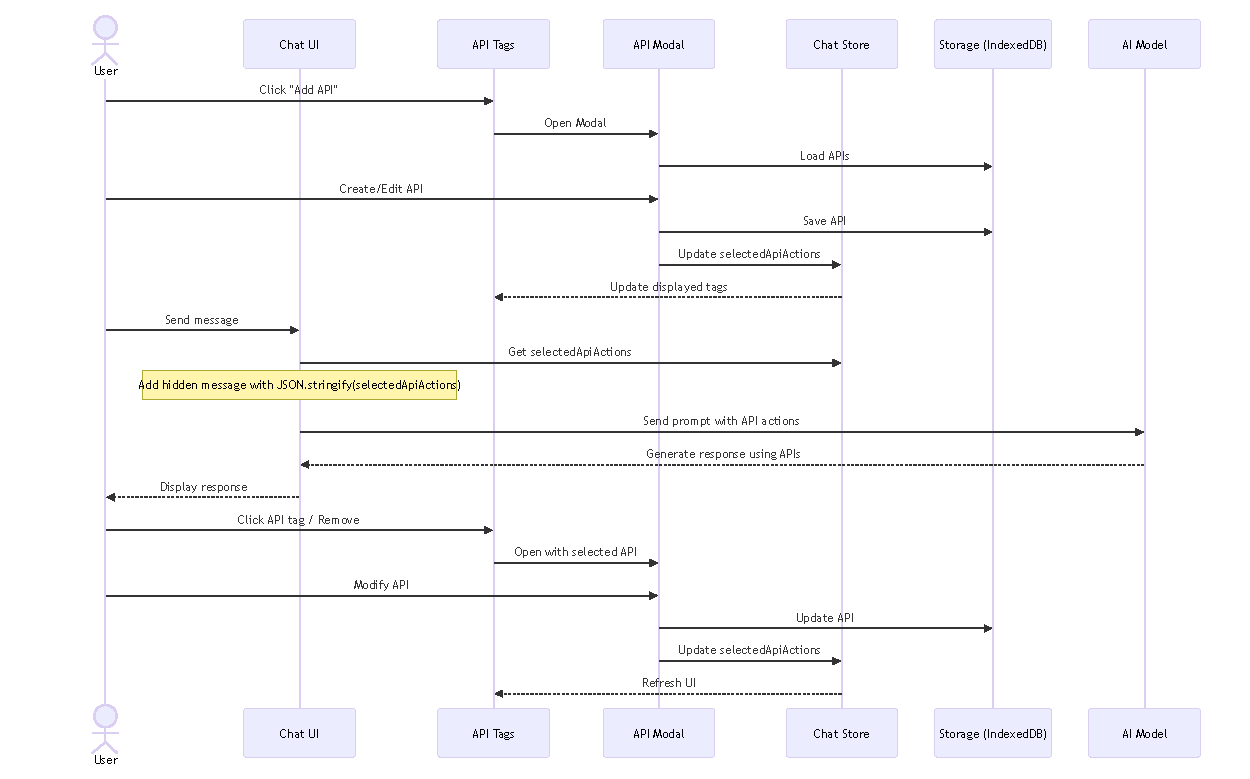
\includegraphics[width=\textwidth]{figures/api_workflow.pdf}
  \caption{API使用工作流程图:展示用户创建、编辑和使用API的完整流程,以及API信息在系统各组件间的传递方式}
  \label{fig:api_workflow}
\end{figure}

\subsection{APIActions与Token效率优化}
在LLM应用开发中,token使用效率是关键考量因素,直接影响系统响应速度、成本和可扩展性。bolt.se的APIActions模块通过OpenAPI规范的结构化定义,提升了token使用效率:

\begin{enumerate}
  \item \textbf{精简上下文传递}:APIActions以结构化格式传递API功能,相比自然语言描述显著节省token消耗。例如,一个包含多个端点的API,结构化的OpenAPI描述比详细自然语言描述需要更少的token。
  
  \item \textbf{减少不确定生成}:通过APIActions,LLM可直接调用外部服务获取准确信息,避免因知识截止限制产生的不确定内容,减少用于生成估计内容的token消耗。
  
  \item \textbf{简化指令结构}:结构化API定义使LLM易于理解可用操作,无需冗长指示说明,节省对话上下文中的token空间。
  
  \item \textbf{减少迭代次数}:清晰的API定义减少LLM理解和使用API所需的交互次数,每减少一轮交互可节省大量token。
\end{enumerate}

在复杂开发任务中,使用APIActions比传统方法减少token消耗,同时提高结果准确性和一致性。这种效率提升对大规模应用部署和持续使用尤为重要,直接降低运营成本。

\subsection{整体架构设计与模块划分}
bolt.se的APIActions系统采用模块化设计,由以下核心组件构成:

\begin{enumerate}
  \item \textbf{用户界面组件}:
    \begin{itemize}
      \item \texttt{ApiActionsContextTags}:显示聊天界面中选中的API标签
      \item \texttt{ApiActionsModal}:管理API的主要模态窗口
      \item \texttt{EditApiActionsModal}:创建和编辑API的编辑器界面
    \end{itemize}
  
  \item \textbf{数据管理组件}:
    \begin{itemize}
      \item \texttt{chatStore}:管理当前聊天中选中的API(selectedApiActions)
      \item \texttt{useApiActions}:提供API增删改查功能的React Hook
      \item \texttt{IndexedDB存储}:持久化存储API定义
    \end{itemize}
  
  \item \textbf{AI交互层}:负责将选定API信息传递给LLM,并处理模型响应结果。
\end{enumerate}

如图\ref{fig:api_workflow}所示,整个API使用流程分为三个主要阶段:API创建与管理、在对话中使用API以及API的编辑与移除。这种设计确保了API的全生命周期管理,从定义到使用再到维护的完整闭环。

在数据模型设计方面,bolt.se定义了结构化的API数据模型,如图\ref{fig:api_actions_class}所示。核心数据结构是ApiActions类,包含API的所有必要信息:

\begin{figure}[htbp]
  \centering
  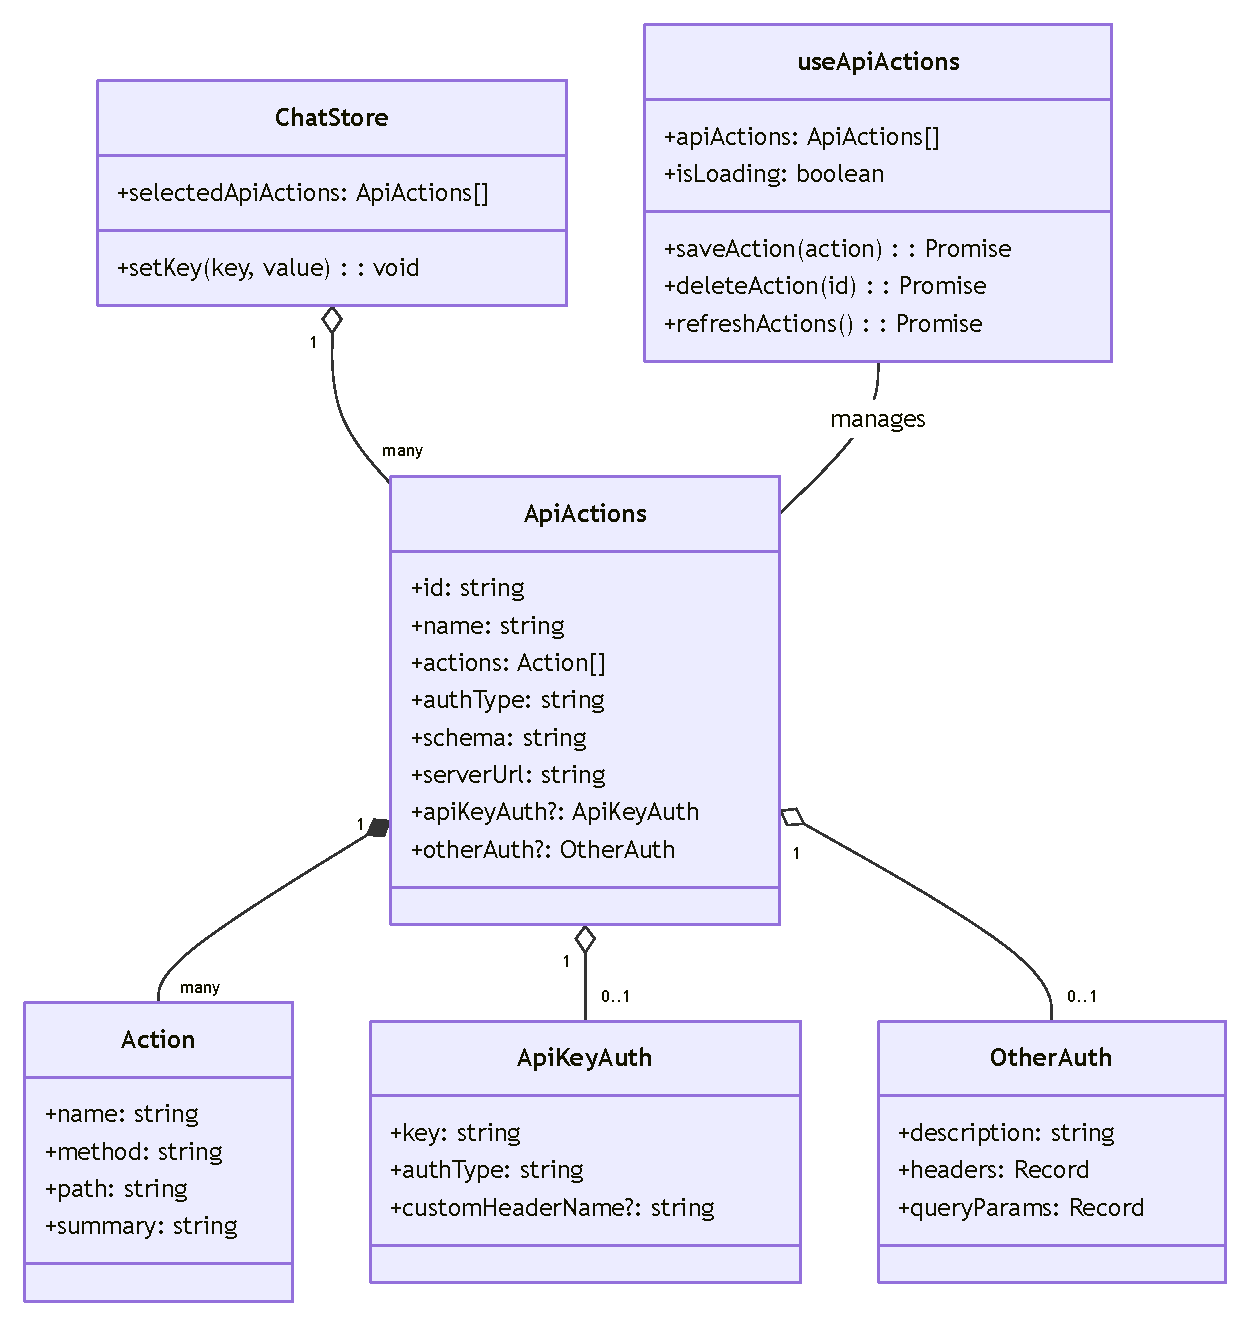
\includegraphics[width=\textwidth]{figures/api_actions_class.pdf}
  \caption{API数据模型类图:描述系统中API定义的核心数据结构及其关系,包括API操作、认证方式和存储管理}
  \label{fig:api_actions_class}
\end{figure}

ApiActions数据模型主要包括:

\begin{enumerate}
  \item \textbf{基本信息}:唯一标识符(id)、名称(name)和基础URL(serverUrl)。
  
  \item \textbf{API操作集}:由多个Action对象组成,每个Action定义一个API端点的HTTP方法、路径和功能摘要。
  
  \item \textbf{认证信息}:支持三种认证方式:
    \begin{itemize}
      \item \texttt{none}:无需认证的API
      \item \texttt{apiKey}:通过API密钥认证,支持Basic、Bearer或自定义头部方式
      \item \texttt{other}:其他自定义认证,可配置自定义头部和查询参数
    \end{itemize}
  
  \item \textbf{OpenAPI规范}:通过schema字段存储完整OpenAPI规范定义,为系统提供API详细信息。
\end{enumerate}

bolt.se的APIActions模块具有以下关键功能:

\begin{enumerate}
  \item \textbf{OpenAPI解析与提取}:系统解析OpenAPI规范,自动识别并提取API端点、方法和参数,减少用户配置负担。
  
  \item \textbf{多种认证支持}:灵活支持不同API认证方式,包括无认证、API密钥(Bearer、Basic、自定义头部)和其他自定义认证方式。
  
  \item \textbf{API标签系统}:通过标签化展示选中API,提供直观视觉反馈,方便管理多个API。
  
  \item \textbf{实时编辑与更新}:支持API定义的实时编辑和更新,变更立即反映在对话中。
  
  \item \textbf{LLM集成机制}:将选中API信息以结构化形式注入LLM上下文,使模型能理解并正确调用这些API。
\end{enumerate}

\section{实例应用场景}

本节以聊天机器人应用为例,展示在bolt.se中如何使用APIActions模块集成多个外部API,并借助LLM实现任务规划、代码生成与界面交互。该机器人能够回答天气相关问题并展示狗狗图片,集成了OpenAI API、NWS Weather API与The Dog API。

\subsection{添加与配置 APIActions}

用户首先通过图形界面进入APIActions模块(如图\ref{fig:demo_edit}),粘贴OpenAPI定义并选择认证方式。以NWS Weather API为例,其提供两个操作端点,分别用于获取经纬度对应的网格点与天气预报:

\begin{figure}[htbp]
  \centering
  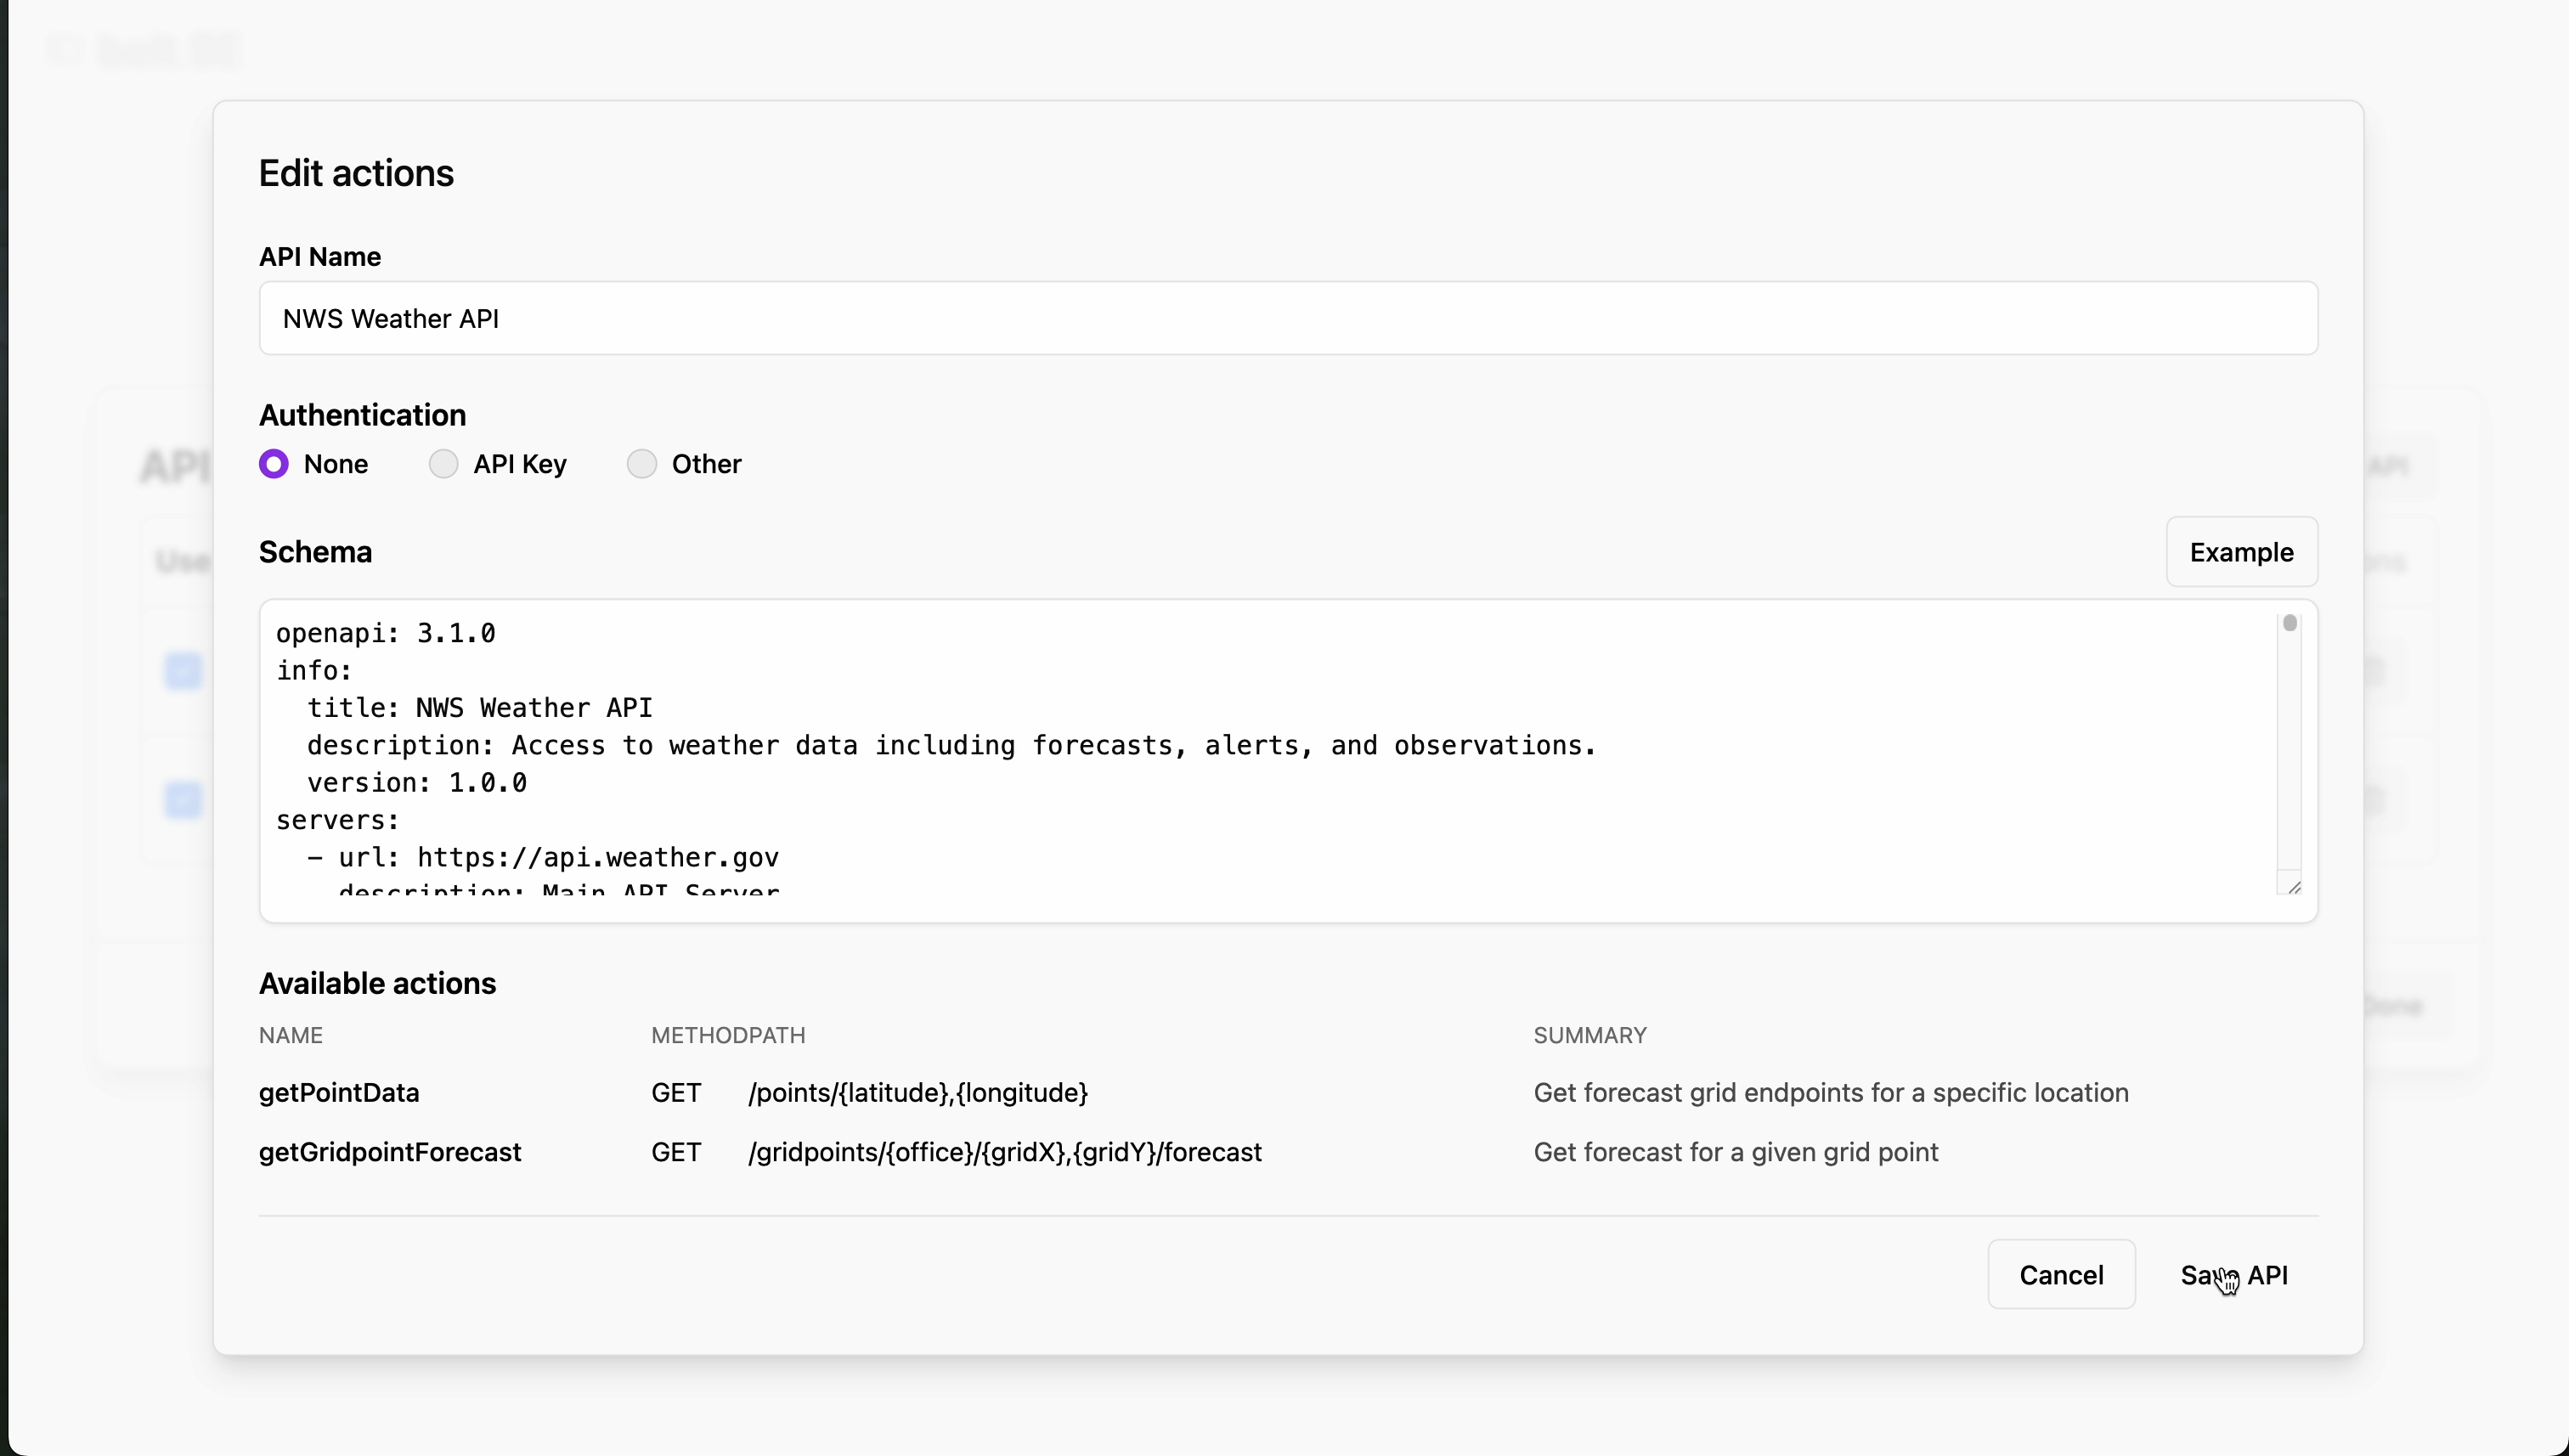
\includegraphics[width=\textwidth]{figures/screenshots/api-actions/demo_edit_modal.png}
  \caption{添加NWS Weather API:通过粘贴OpenAPI规范定义并配置端点与认证方式}
  \label{fig:demo_edit}
\end{figure}

配置完成后,用户可在APIActions列表中启用或禁用对应API,系统支持随时编辑、删除、重载schema(如图\ref{fig:demo_table})。

\begin{figure}[htbp]
  \centering
  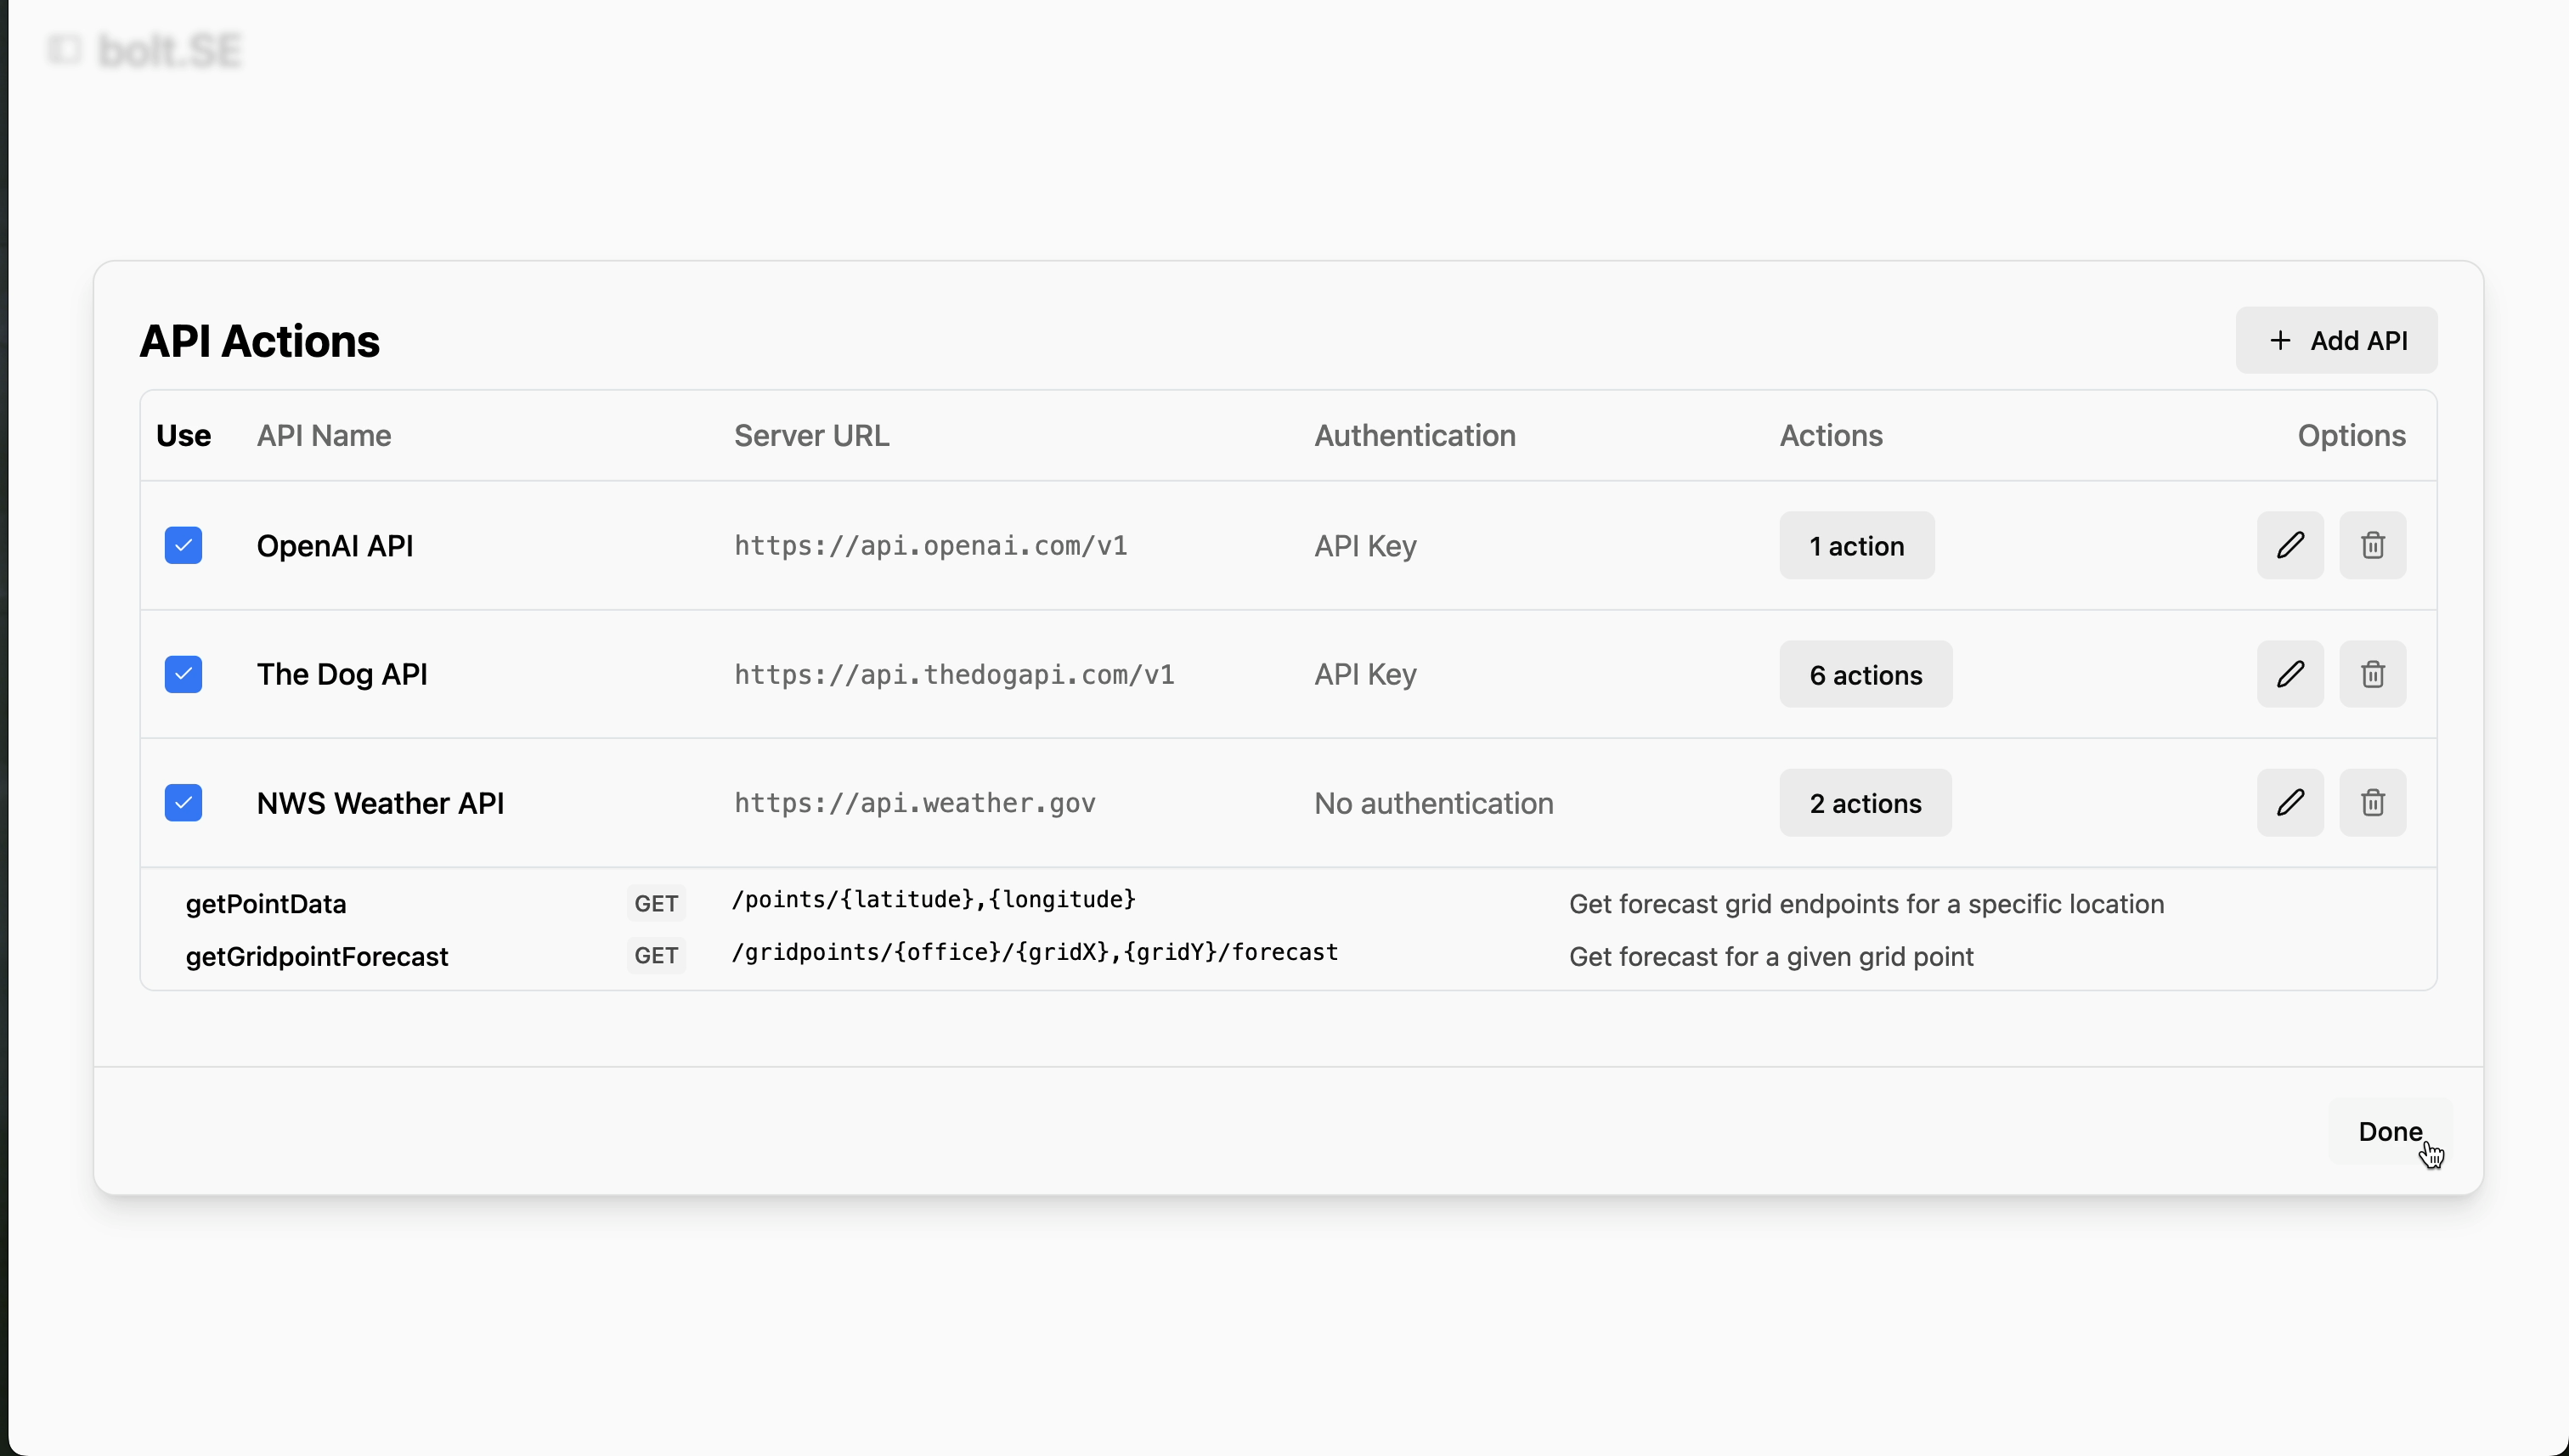
\includegraphics[width=\textwidth]{figures/screenshots/api-actions/demo_actions_table.png}
  \caption{APIActions总览界面:展示所有注册的API、认证方式与可用操作数}
  \label{fig:demo_table}
\end{figure}

\subsection{自然语言触发任务规划与代码生成}

完成API配置后,用户可在主对话框中勾选所需API(如图\ref{fig:demo_prompt}),并以自然语言输入构想,例如:

\begin{quote}
\texttt{make a chatbot that can answer weather related questions and show dog images}
\end{quote}

\begin{figure}[htbp]
  \centering
  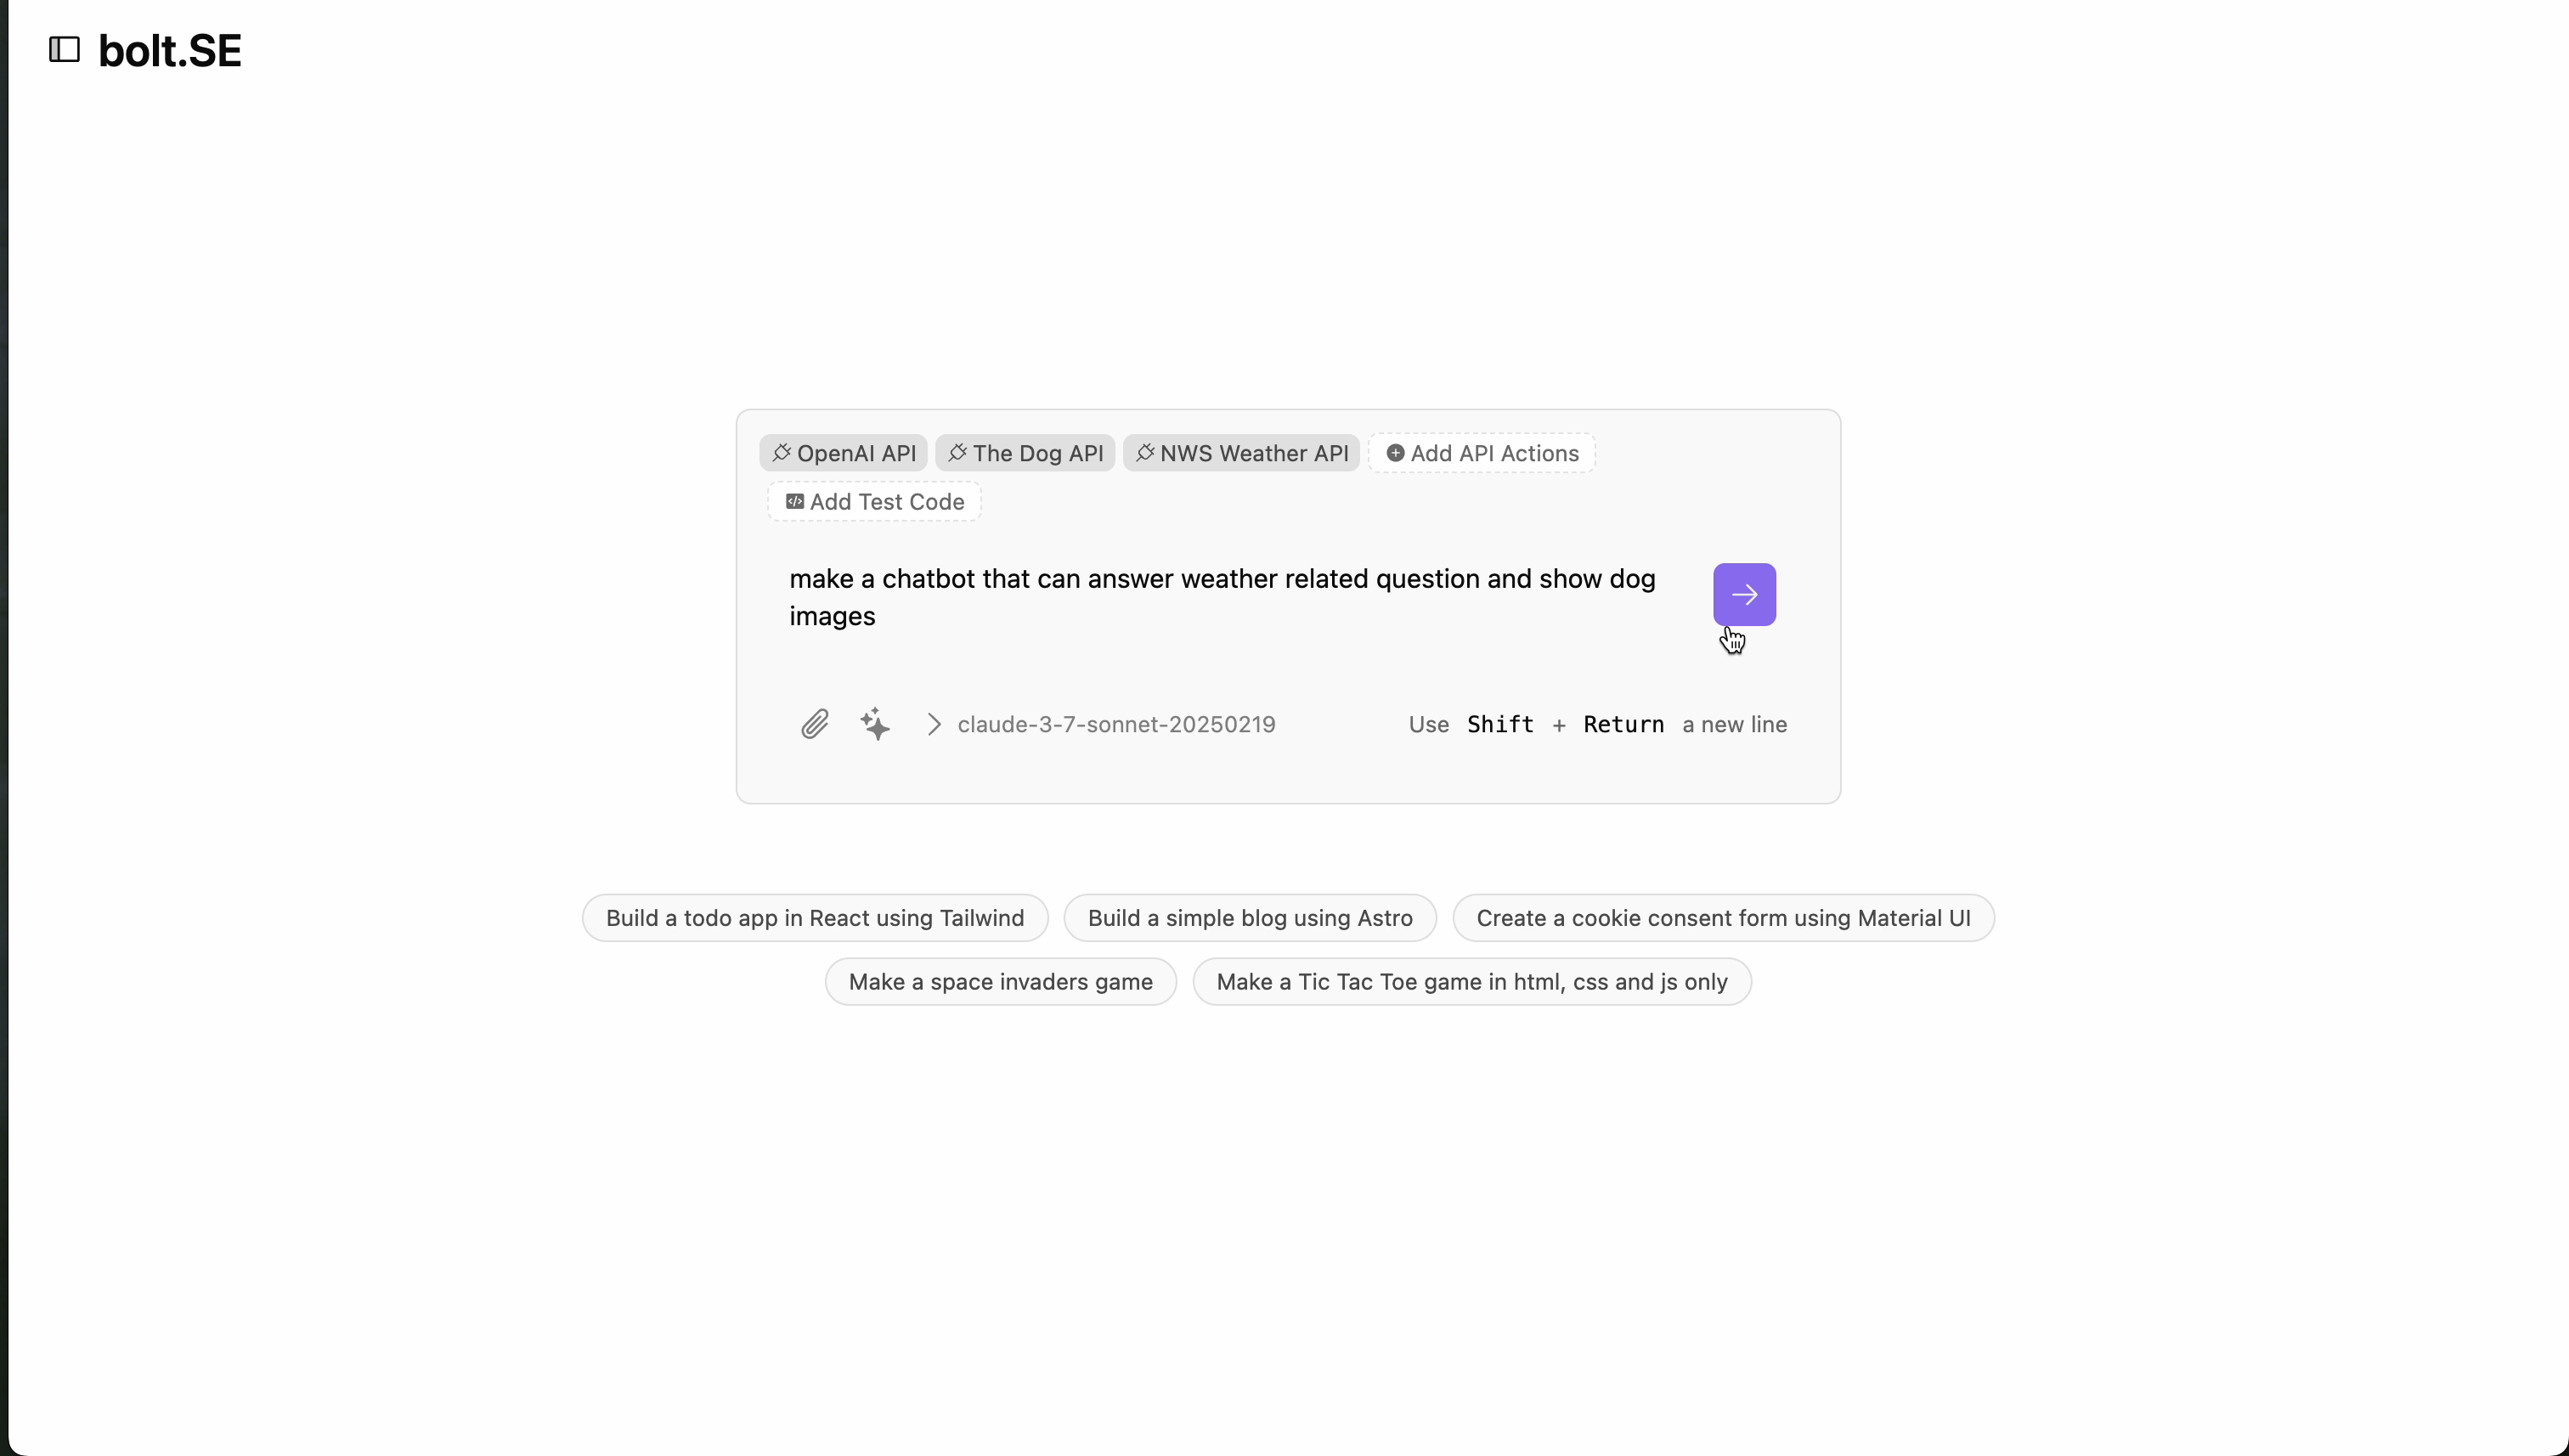
\includegraphics[width=\textwidth]{figures/screenshots/api-actions/demo_prompt_tags.png}
  \caption{对话框中勾选相关API,配合自然语言指令触发任务生成}
  \label{fig:demo_prompt}
\end{figure}

系统基于勾选的API及用户意图,自动规划任务、生成文件,并提示相关操作步骤。

\subsection{代码结构与依赖初始化}

如图\ref{fig:demo_plan}所示,bolt.se自动列出开发计划并创建必要文件结构,同时生成项目依赖清单与安装命令。

\begin{figure}[htbp]
  \centering
  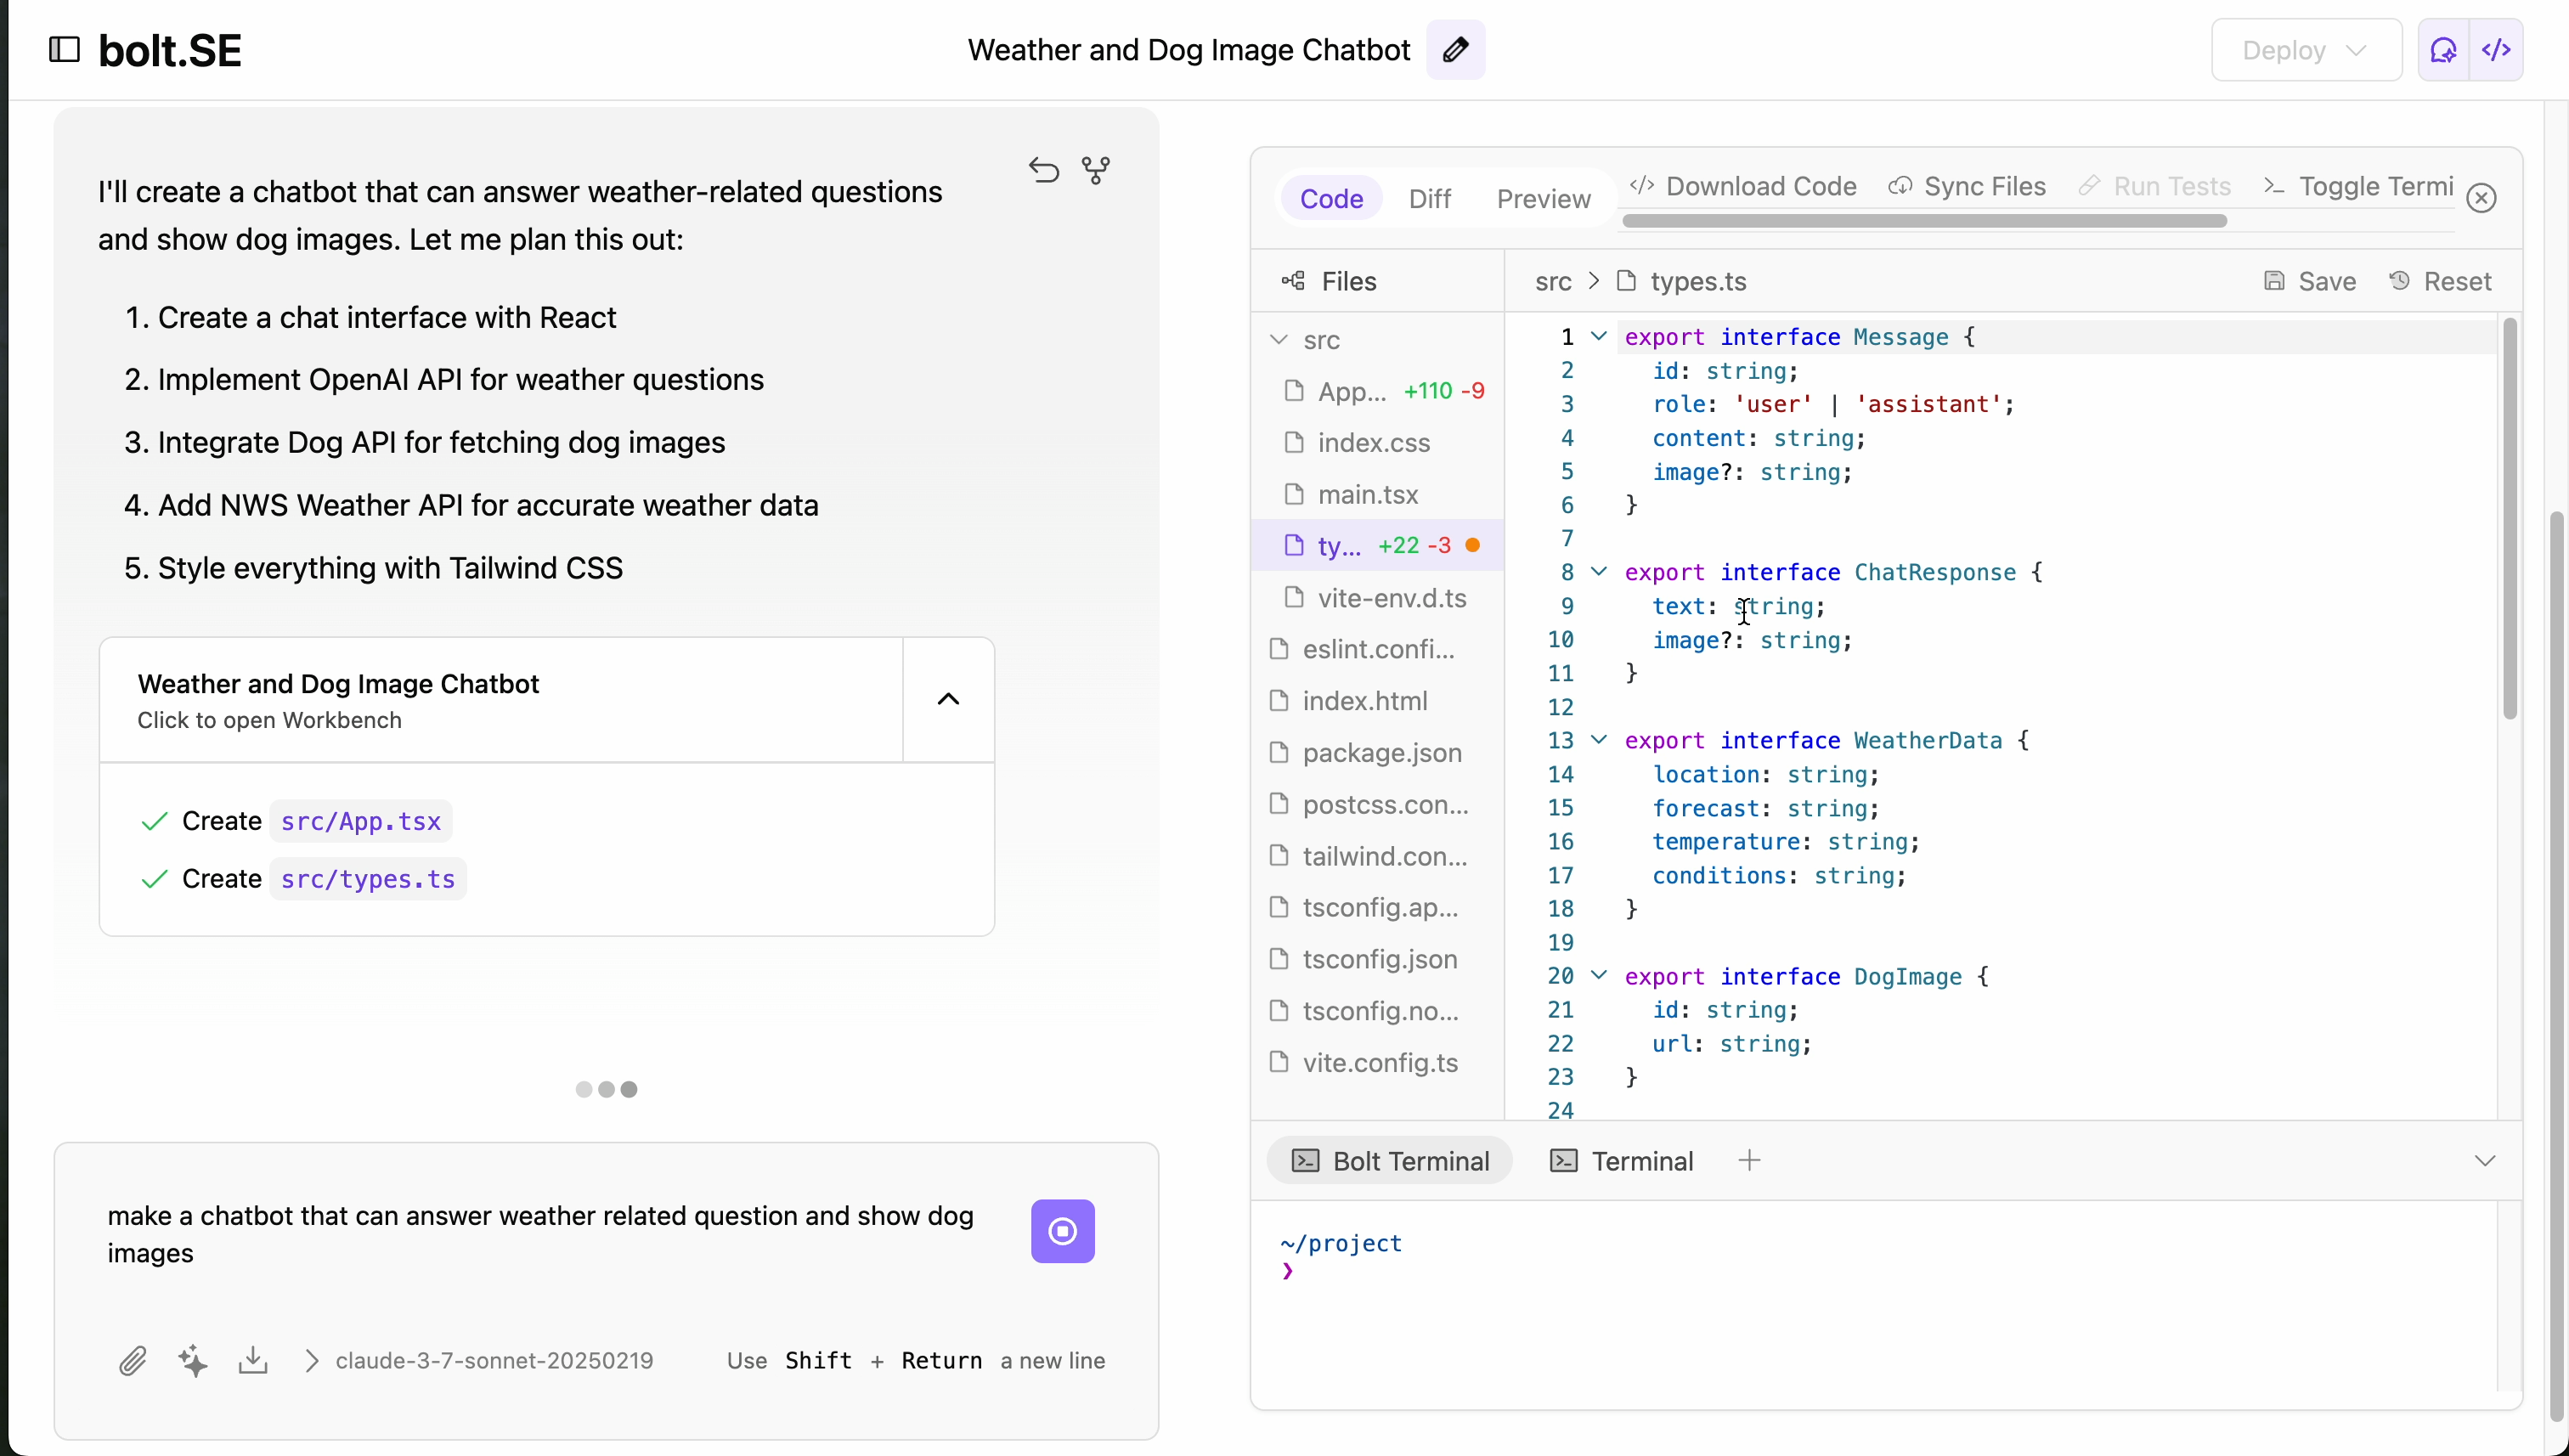
\includegraphics[width=\textwidth]{figures/screenshots/api-actions/demo_plan_files.png}
  \caption{系统生成项目结构与依赖安装命令,覆盖前端组件与服务调用逻辑}
  \label{fig:demo_plan}
\end{figure}

\subsection{交互效果与API调用验证}

在预览界面中,用户可实时测试机器人功能:

\begin{figure}[htbp]
  \centering
  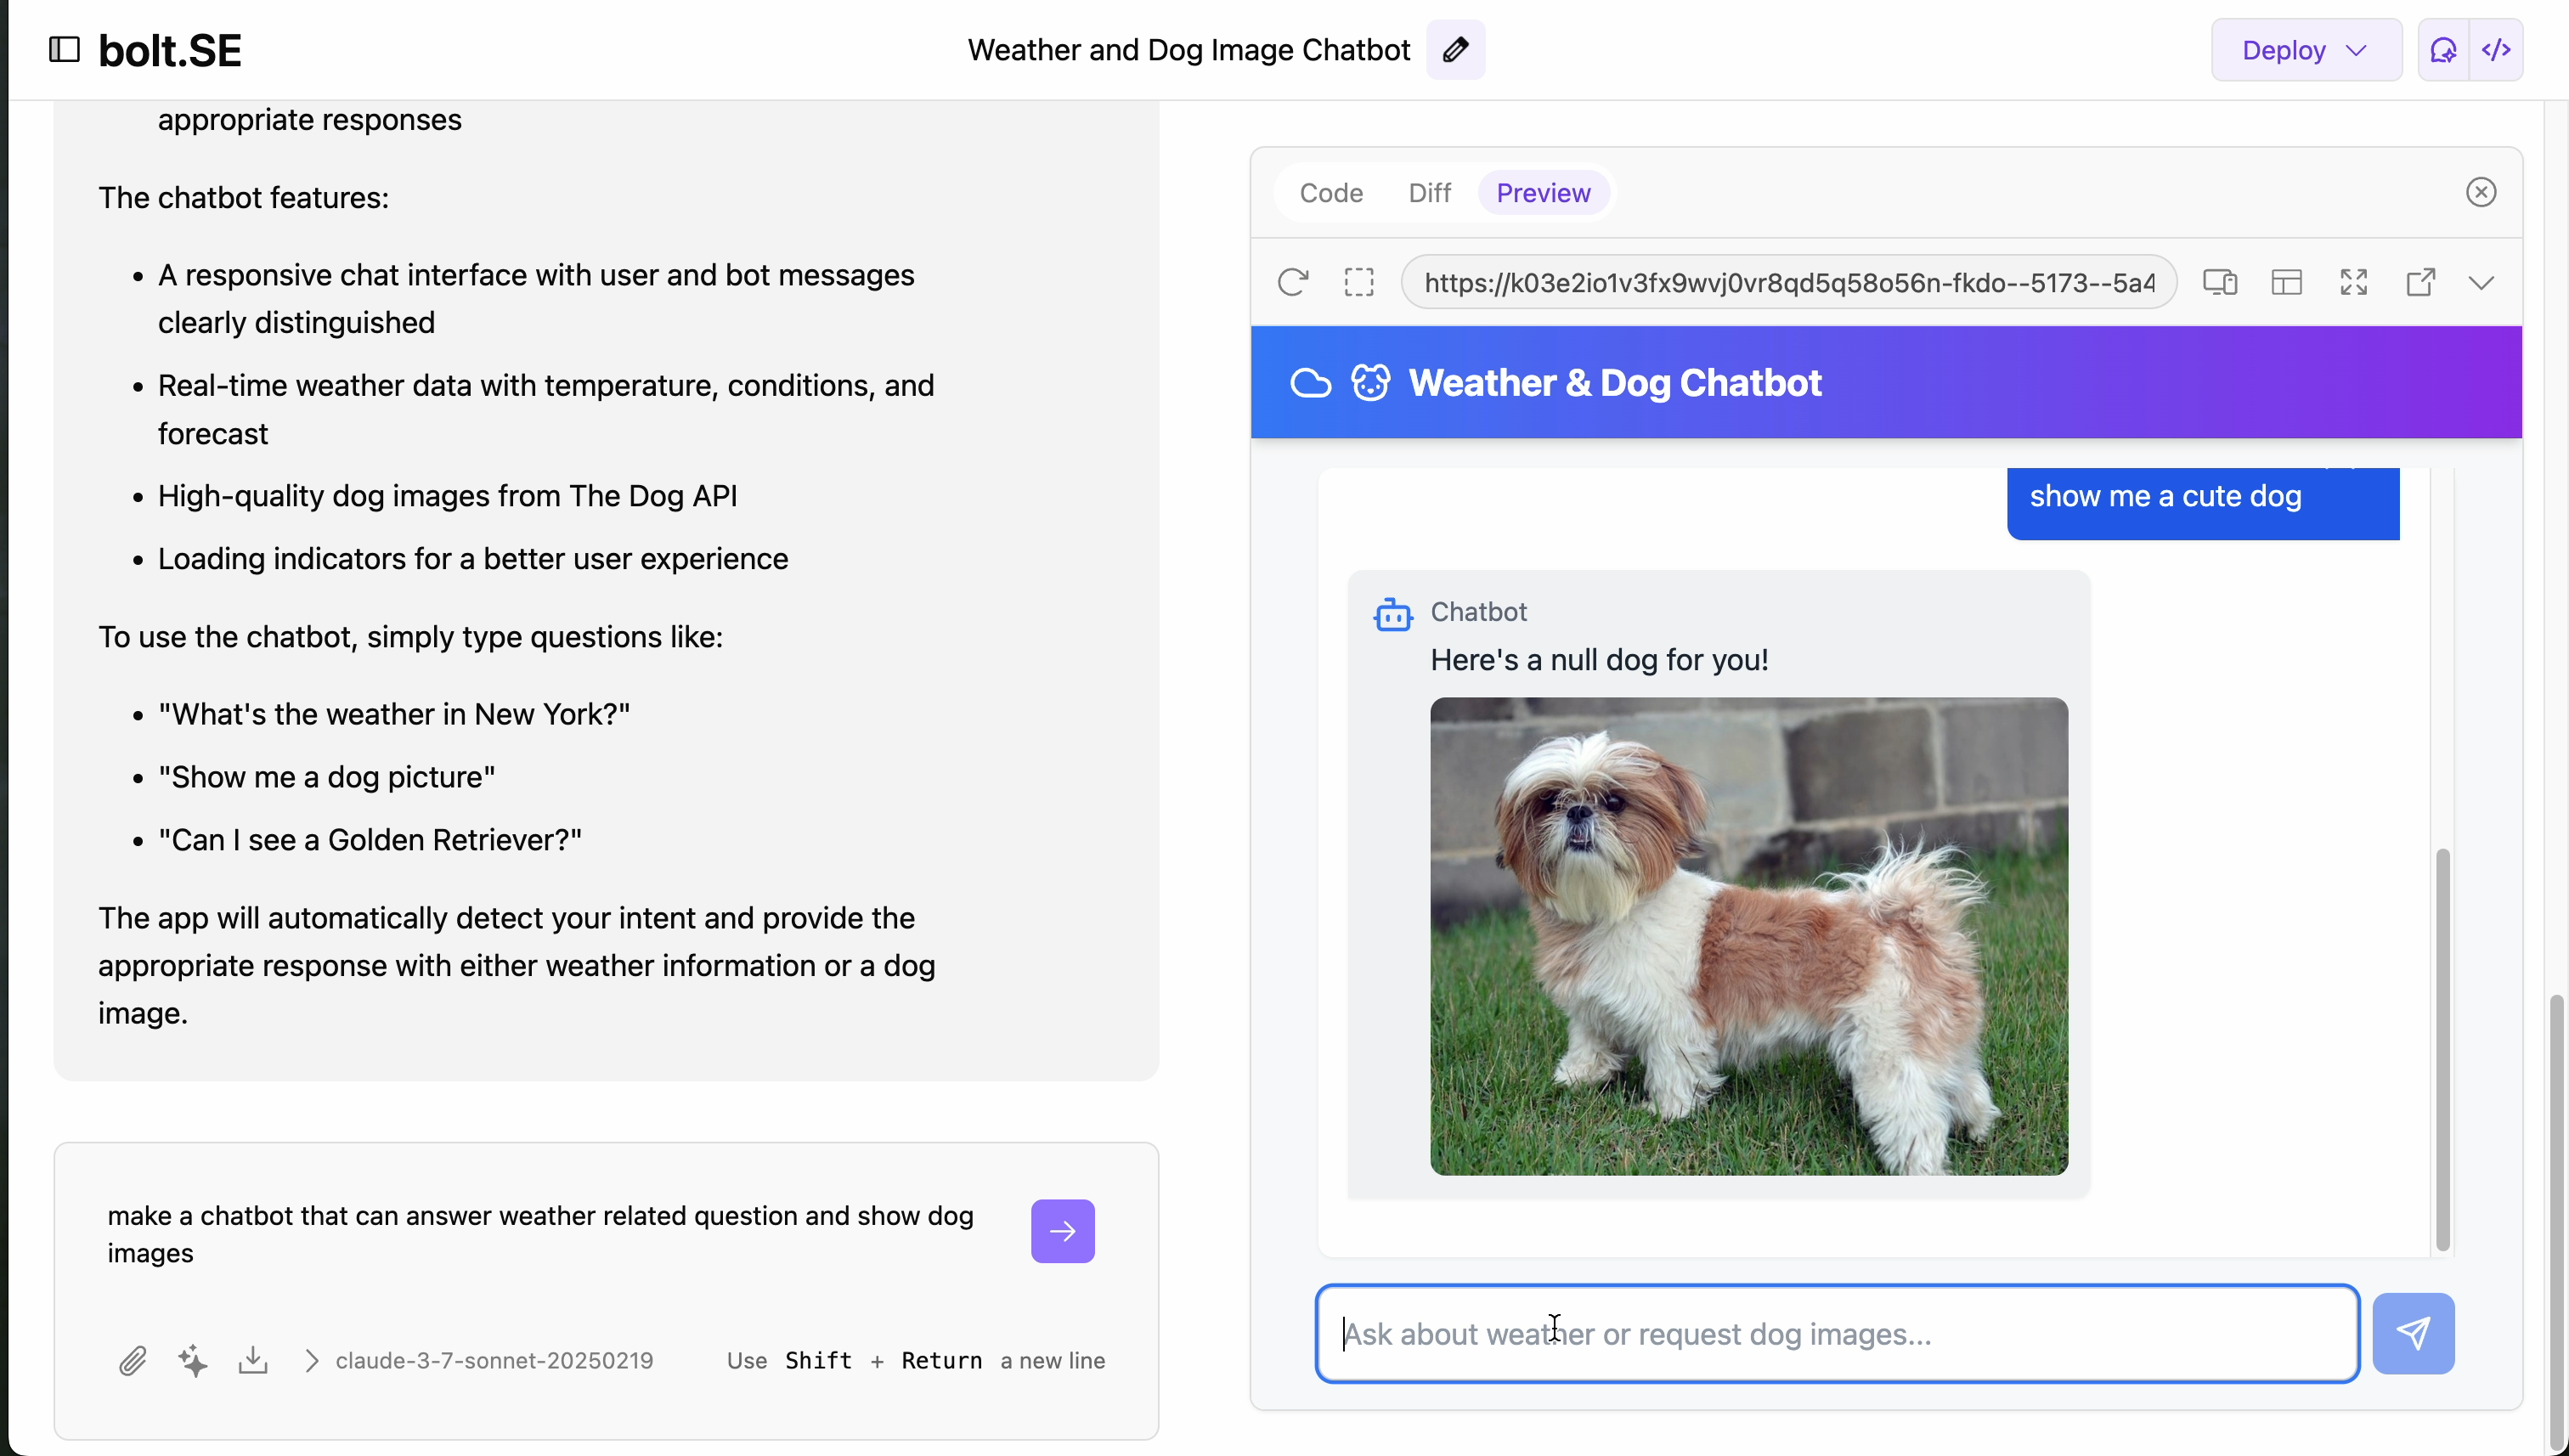
\includegraphics[width=\textwidth]{figures/screenshots/api-actions/demo_dog_preview.png}
  \caption{用户请求"show me a cute dog",系统调用The Dog API返回图片}
  \label{fig:demo_dog}
\end{figure}

\begin{figure}[htbp]
  \centering
  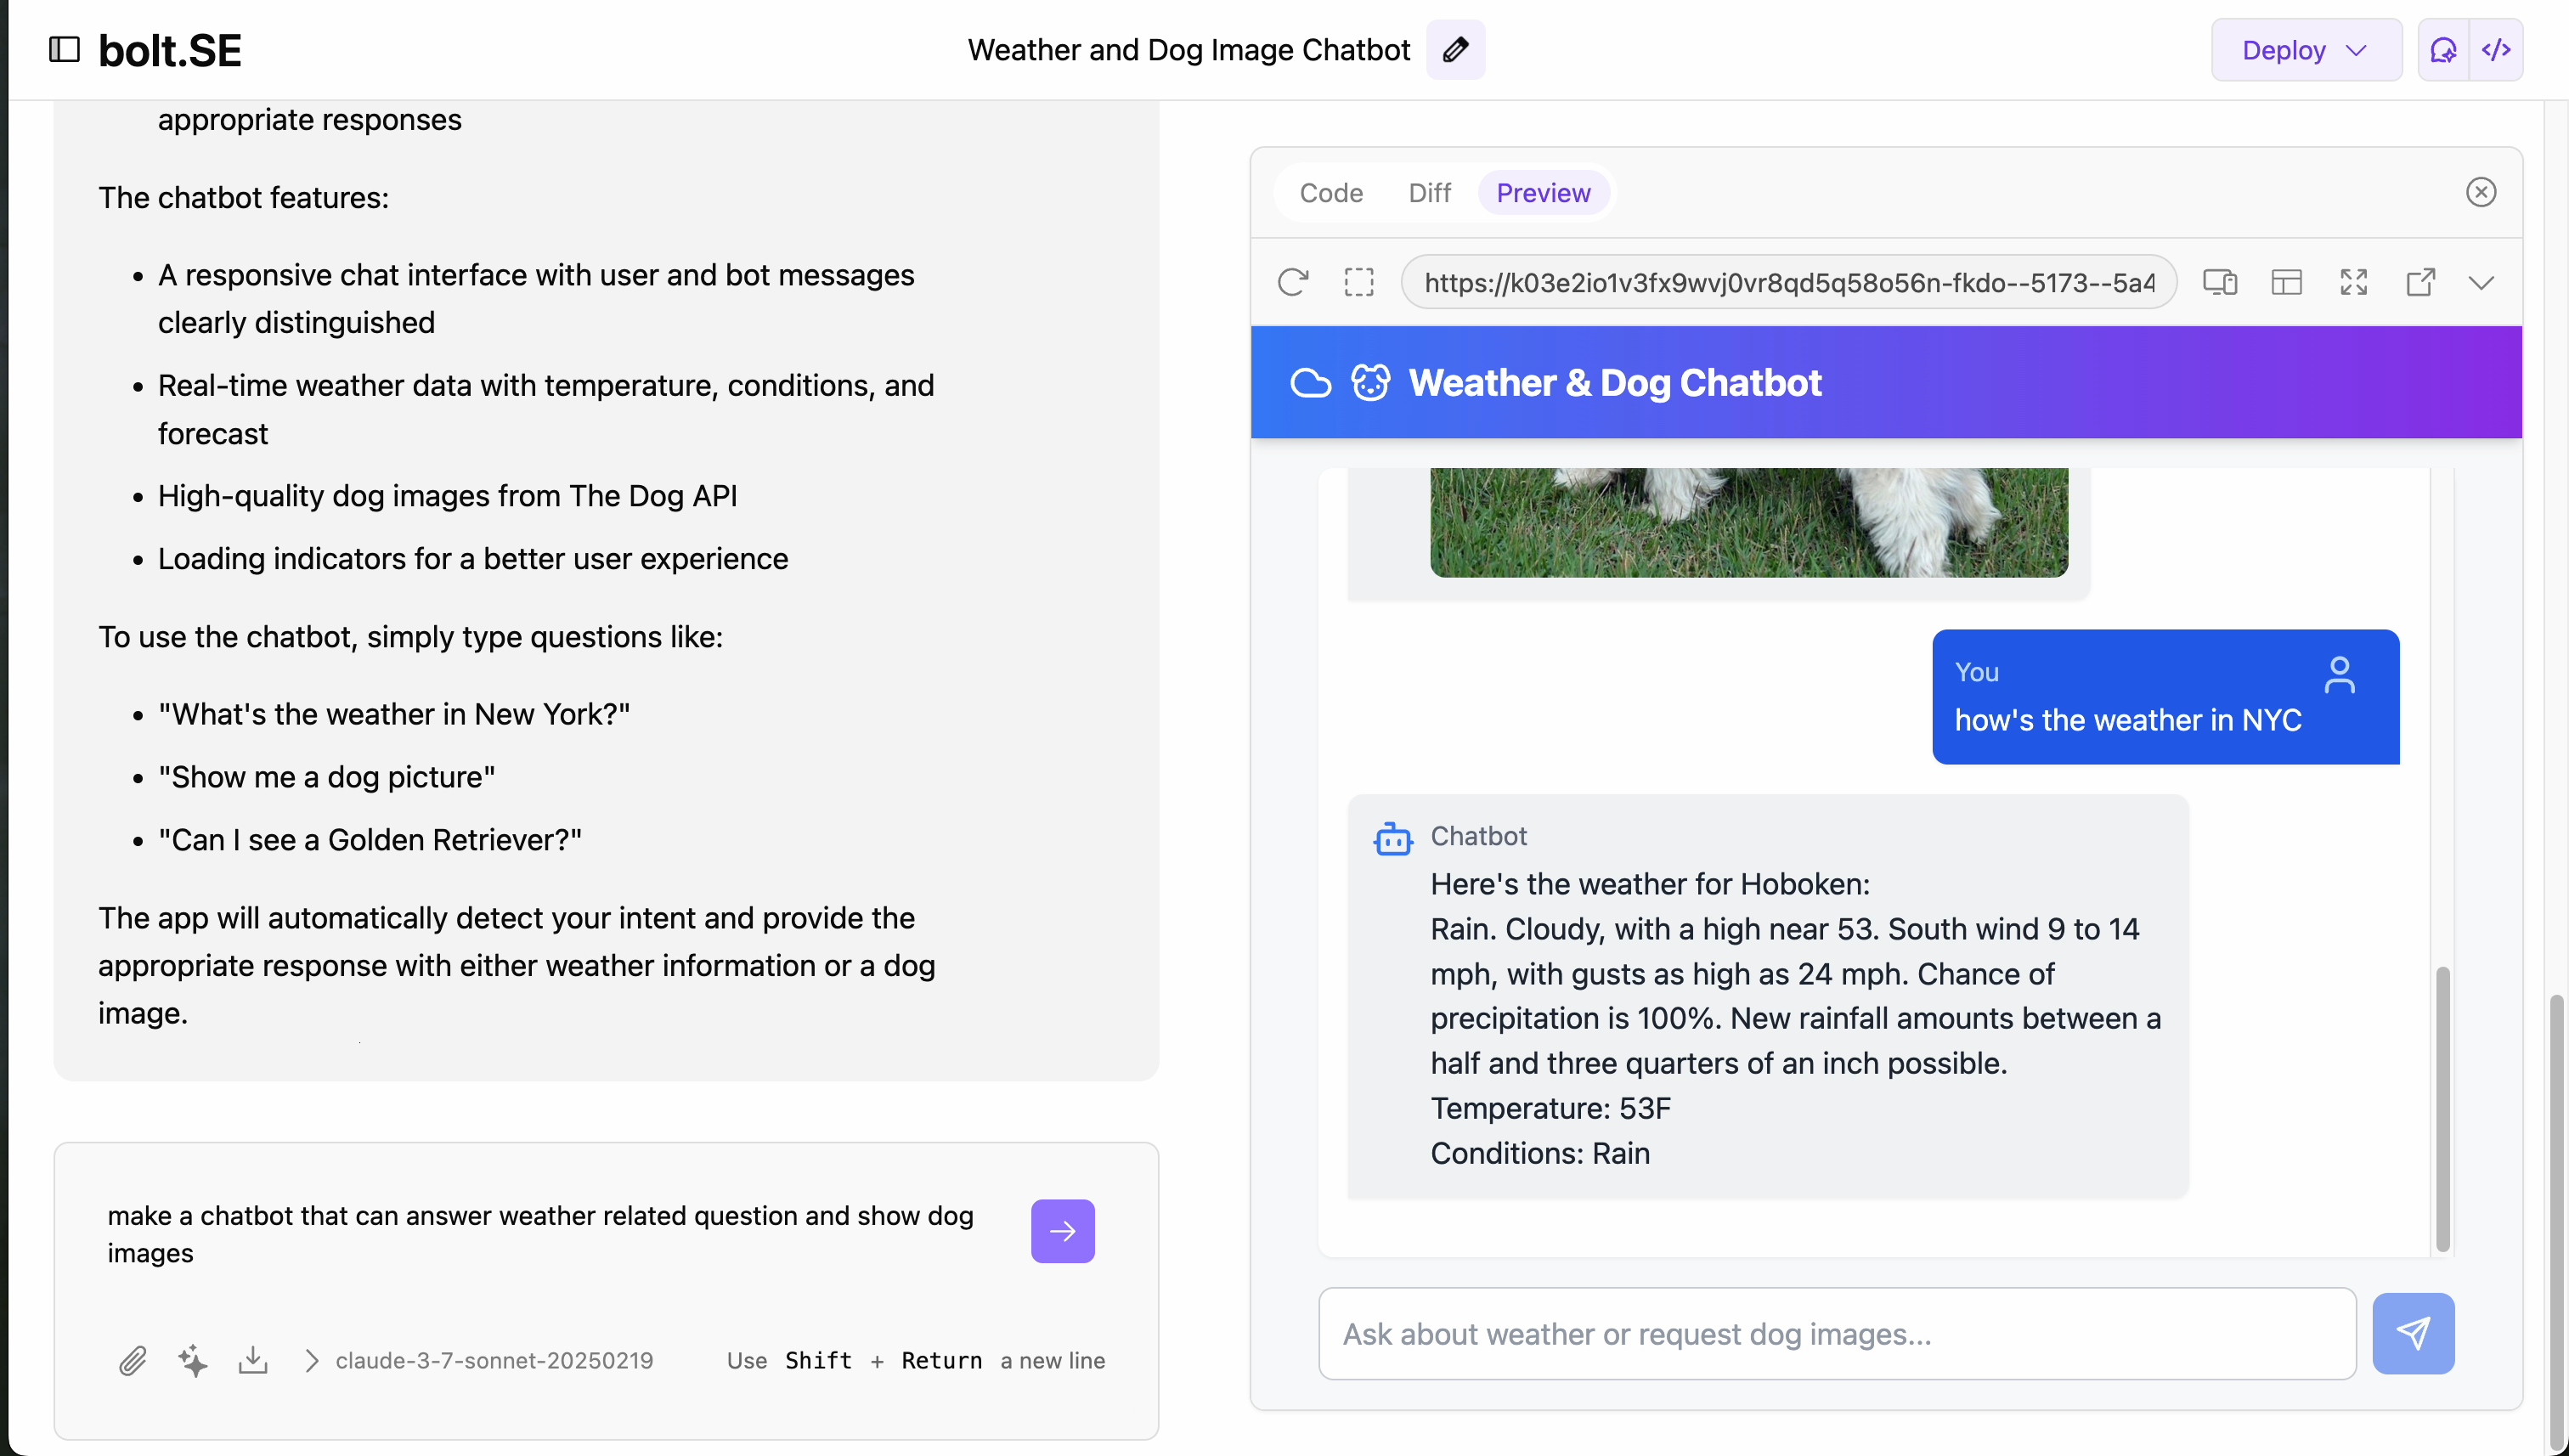
\includegraphics[width=\textwidth]{figures/screenshots/api-actions/demo_weather_preview.png}
  \caption{询问天气时,系统识别意图并调用NWS Weather API提供实时天气信息}
  \label{fig:demo_weather}
\end{figure}

从图中可见,聊天机器人能准确识别用户意图,并将意图转化为对外部API的调用,展示了APIActions与LLM的协同优势。

\subsection{与传统开发方式对比}

API优先开发方式与传统开发相比具有以下优势:

\begin{itemize}
  \item \textbf{集成效率}:传统开发需手动编写API调用代码与参数处理逻辑,而APIActions仅需粘贴OpenAPI文档即可自动生成。
  
  \item \textbf{token节省}:结构化API定义避免冗长自然语言说明,显著降低上下文长度。OpenAPI规范作为结构化格式,比传统开发中的自然语言描述可节省大量token消耗。 
  
  \item \textbf{开发误差减少}:系统自动完成接口字段绑定,避免路径拼写、参数顺序或认证机制的人工错误。
  
  \item \textbf{上下文利用率提升}:传统方法中,大量token用于描述API功能和使用方法,而API优先方法通过结构化定义减少冗余信息,使有限token更多用于实际问题解决。
  
  \item \textbf{减少交互轮次}:由于API定义明确,LLM能一次性正确理解和使用API,减少多轮交互纠错,每减少一轮交互可节省大量token。
\end{itemize}

API优先模式在涉及复杂外部服务集成的场景中,不仅提高开发效率和应用质量,同时通过结构化API描述和减少交互轮次,显著降低LLM应用的token消耗和运营成本。
